\documentclass{article}

\usepackage[final]{style}
\usepackage[utf8]{inputenc} % allow utf-8 input
\usepackage[T1]{fontenc}    % use 8-bit T1 fonts
\usepackage{hyperref}       % hyperlinks
\usepackage{url}            % simple URL typesetting
\usepackage{booktabs}       % professional-quality tables
\usepackage{amsfonts}       % blackboard math symbols
\usepackage{nicefrac}       % compact symbols for 1/2, etc.
\usepackage{microtype}      % microtypography
\usepackage{verbatim}
\usepackage{graphicx}       % for figures

\title{Lecture \#6: Reconstrução 3D: Formas a partir de sombra, estéreo, textura e foco. Detecção de profundidade usando sensores ativos. Representação de superfícies e reconstrução baseada em modelos.}

\author{
  Felipe Torres Minorelli, Kevin Perondi Regis, Renan Viana Hoshi \\
  Department of Computer Science\\
  Federal University of Technology - Paran\'{a} / UTFPR\\
  Campo Mour\~{a}o, Paran\'{a}, Brazil \\
  \texttt{\{felipeminorelli,kevinperondi,renanvianah\}@gmail.com} \\
}

\begin{document}

\maketitle


\section{Introdução}

bla bla bla

\section{Formas a partir de sombra, estéreo, textura e foco}

Neste capítulo realizaremos o estudo de como formas podem ser inferidas a partir do sombreamento, textura e foco. Assim como estas 3 instâncias podem ser utilizadas para a reconstrução da geometria de um objeto 3D.

\subsection{Formas a partir de sombra}

Ao se observar um objeto sombreado, podemos distinguir sua forma apenas com a variação de sombreamento. Tal fenômeno ocorre pois a superfície normal do objeto muda ao longo de seu exterior, desta forma temos uma variação do brilho já que o mesmo é decorrente entre a variação da orientação da superfície e o ângulo da iluminação incidente. Podemos observar estas mudanças na Figura~\ref{fig:sombra}.

\begin{figure}[!htb]
    \centering
    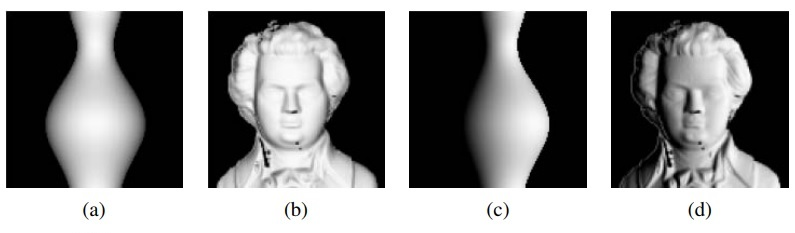
\includegraphics[width=0.90\textwidth]{imagem1.jpg}
    \caption{Forma sintética a partir de sombreamento (Zhang, Tsai, Cryer et al. 1999)}
    \label{fig:sombra}
\end{figure}

A recuperação da forma de uma superfície a partir desta variação é conhecida como \textit{shape from shading}, é um problema recorrente em visão computacional.
A maioria dos algoritmos de sombreamento assumem que o coeficiente de reflexão seja uniforme, e as direções da fonte de luz sejam conhecidas ou passiveis de alterações pelo uso de um objeto de referencia. A partir das suposições de observador e fontes de luz distantes, a variação de intensidade (equação de irradiância, Figura \ref{eq:irrad}) é baseada na orientação da superfície, onde (p,q) = (zx,zy) são as derivadas do mapa de profundidade e R(p,q) é o chamado mapa de reflectância.

\begin{figure}[!htb]
    \centering
    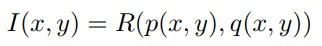
\includegraphics[width=0.60\textwidth]{equacao1.jpg}
    \caption{Equação de irradiância}
    \label{eq:irrad}
\end{figure}

Por exemplo uma superfície difusa, tem um mapa de reflectância calculado através do produto entre um ponto não negativo e a superfície normal e a direção da fonte de luz, Figura \ref{eq:mapareflec}, onde \textit{p} é é o fator de reflectância da superfície.

\begin{figure}[!htb]
    \centering
    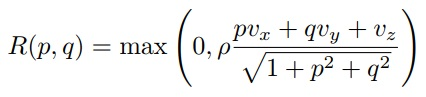
\includegraphics[width=0.60\textwidth]{equacao2.jpg}
    \caption{Equação do mapa de reflectância}
    \label{eq:mapareflec}
\end{figure}

Teoricamente as equações \ref{eq:irrad} e \ref{eq:mapareflec} podem ser utilizadas para se estimar (p,q), porém,  a não ser que outras restrições sejam adicionadas, ainda temos mais pares desconhecidos (p,q) do que intensidades calculadas (I). Uma das restrições mais utilizadas é a restrição de suavidade, Figura~\ref{eq:suavidade}. A outra é a restrição de integrabilidade, Figura~\ref{eq:integrabilidade}, onde para uma mapa de profundidade válido temos \textit{z(x,y)} com \textit{(p,q) = (zx,zy)}, portanto \textit{py = zxy = zyx = qx}.

\begin{figure}[!htb]
    \centering
    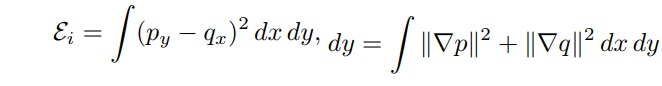
\includegraphics[width=0.60\textwidth]{equacao3.jpg}
    \caption{Restrição de suavidade}
    \label{eq:suavidade}
\end{figure}

\begin{figure}[!htb]
    \centering
    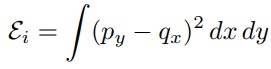
\includegraphics[width=0.60\textwidth]{equacao4.jpg}
    \caption{Restrição de integrabilidade}
    \label{eq:integrabilidade}
\end{figure}

Em vez de primeiro recuperar os campos de orientação \textit{(p, q)} e integrá-los para obter um
superfície, também é possível minimizar diretamente a discrepância na equação de formação de imagem
\ref{eq:irrad} ao encontrar o mapa de profundidade ideal \textit{z (x, y)}. Infelizmente, a forma
a partir do sombreamento é suscetível aos mínimos locais no espaço de busca, e como outros
problemas que envolvem a estimativa simultânea de muitas variáveis, também podem sofrer uma lenta convergência. Para diminuir este problema podemos nos utilizar de técnicas como a de multi-resolução (Szeliski 1991a) para acelerar a convergência, e as técnicas de otimização mais sofisticadas (Dupuis and Oliensis 1994), para a evitar mínimos locais.

Na prática, superfícies diferentes de modelos de gesso raramente possuem um coeficiente de reflectância uniforme. Portanto a reconstrução de forma a partir de sombreamento precisa ser combinado com alguma outra técnica ou estendido de alguma maneira para ter alguma utilidade. Uma maneira de fazer isso é a combinação com a correspondência estéreo (Fua e Leclerc 1995) ou textura conhecida (padrões de superfície) (White e Forsyth 2006), técnicas abordadas nas próximas seções. O estéreo e as componentes de textura fornecem informações em regiões texturizadas, enquanto a forma a partir de sombreamento ajuda preencha as informações em regiões uniformemente coloridas e também fornece informações mais detalhadas sobre a forma da superfície.

\subsection{Formas a partir do estéreo fotométrico}


Outra maneira de tornar a forma a partir do sombreamento mais confiável é utilização de várias
fontes de luz, que podem ser ativadas e desativadas seletivamente. Essa técnica é chamada de estéreo fotométrico. Uma vez que as fontes de luz desempenham um papel análogo às câmeras localizadas em diferentes locais, para cada fonte de luz, temos um mapa de refletância, \textit{R1 (p, q)}, \textit{R2 (p, q)}, etc, assim como as intensidades correspondentes \textit{I1}, \textit{I2}, etc. Em um pixel, podemos, em princípio, recuperar um coeficiente de reflectância desconhecido \textit{p} e uma orientação de superfície estimada \textit{(p, q)}. Para superfícies difusas (equação \ref{eq:mapareflec}), se parametrizarmos a orientação local por  \textit{nˆ}, obtemos (por pixeis não-sombreados) um conjunto de equações lineares da seguinte forma:

\begin{figure}[!htb]
    \centering
    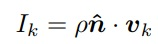
\includegraphics[width=0.3\textwidth]{equacao5.jpg}
    \label{eq:estereo}
\end{figure}

A partir do qual podemos recuperar \textit{pnˆ} usando mínimos quadrados lineares. Essas equações estão bem condicionadas desde que os vetores (três ou mais) \textit{vk} sejam linearmente independentes, isto é, não sejam
ao longo do mesmo azimute (direção oposta do observador). Uma vez que os normais ou gradientes da superfície tenham sido recuperados em cada pixel, eles podem ser integrado em um mapa de profundidade usando uma variante de ajuste de superfície regularizado. 

Quando as superfícies são especulares, podem ser necessárias mais de três direções de luz. De fato,
a equação de irradiância dada na Figura~\ref{eq:irrad} não requer apenas que as fontes de luz e a câmera sejam
distante da superfície, mas também negligencia as inter-reflexões, que podem ser uma fonte significativa
do sombreamento observado nas superfícies dos objetos, por exemplo, o escurecimento visto dentro das estruturas côncavas como ranhuras e fendas.

\subsection{Formas a partir da textura}

A variação no escorço observado em texturas regulares também pode fornecer informações úteis sobre a orientação da superfície local. Na Figura\ref{fig:textura} temos um exemplo desse padrão, ao longo
com as orientações de superfície locais estimadas. Algoritmos de formas a partir de textura requerem um número
etapas de processamento, incluindo a extração de padrões repetidos ou a medição de frequências para calcular deformações afins locais, e um estágio subsequente para inferir orientação de superfície.

\begin{figure}[!htb]
    \centering
    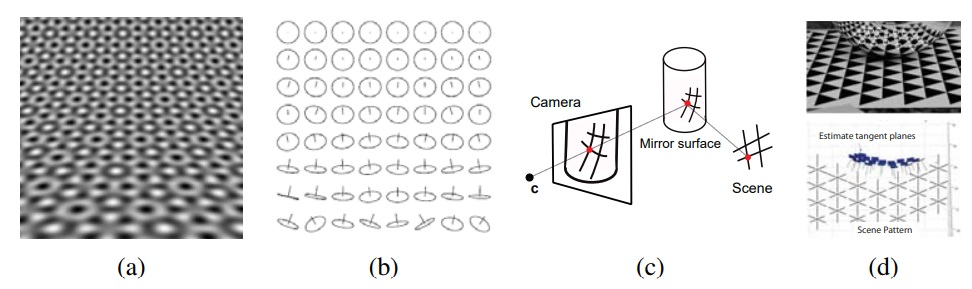
\includegraphics[width=0.9\textwidth]{imagem2.jpg}
    \caption{Forma sintética a partir da textura (Garding 1992)}
    \label{fig:textura}
\end{figure}


Quando o padrão original é regular, é possível ajustar um padrão regular, mas ligeiramente deformado, e usar essa grade para uma variedade de tarefas de substituição ou análise de imagens. Este processo torna-se ainda
mais fácil se padrões de tecido texturizado especialmente impressos forem usados. As deformações induzidas em um padrão regular, quando vistas na reflexão de um espelho curvo, como mostrado na Figura~\ref{fig:textura}, podem ser utilizadas para a recuperação da forma da superfície. Também é possível inferir informações de formas locais a partir do fluxo especular, ou seja, o movimento de especularidades quando visto de uma câmera em movimento.

\subsection{Formas a partir do foco}


Uma boa dica sobre a profundidade de um objeto é a quantidade de desfoque, que aumenta à medida que a superfície do objeto se afasta da distância de focagem da câmera. Movendo-se a superfície de um objeto para longe do plano de foco, aumentamos assim o círculo de confusão, quando calculado a partir de uma fórmula,podemos estabelecer esta característica facilmente.

Várias técnicas foram desenvolvidas para estimar a profundidade a partir da quantidade de desfocagem (profundidade de desfocagem) (Pentland 1987; Nayar and Nakagawa 1994; Nayar, Watanabe,
and Noguchi 1996; Watanabe and Nayar 1998; Chaudhuri and Rajagopalan 1999; Favaro
and Soatto 2006). Mas para que estas técnicas sejam efetivas é necessário levar em conta os seguintes problemas: 

\begin{enumerate}
    \item A quantidade de desfoque aumenta em ambas as direções à medida que você se afasta do plano de foco. Portanto, é necessário usar duas ou mais imagens capturadas com diferentes configurações de distância de foco, ou realizar a transformação das profundidades do objeto e analisar o ponto de nitidez máxima.
    \item A ampliação do objeto pode variar conforme a distância do foco é alterada ou o objeto é movido. Isso pode ser modelado explicitamente (tornando a correspondência mais difícil) ou a partir do uso da óptica telecêntrica, que aproxima uma câmera ortográfica e requer uma abertura na frente da lente.
    \item A quantidade de desfocagem deve ser estimada de maneira confiável. Uma abordagem simples é calcular a média quadrada do gradiente em uma região, mas tal abordagem pode sofrer de vários problemas, incluindo o problema de ampliação da imagem mencionado acima. Uma solução melhor é utilização de filtros racionais.

\end{enumerate}




\section{Detecção de profundidade usando sensores ativos}

bla bla bla

\section{Representação de superfícies}

bla bla bla

\section{Reconstrução baseada em modelos}

bla bla bla

% References
\small
\bibliographystyle{plain}
\bibliography{bibliography}
\end{document}

